\documentclass[11pt]{article}
\usepackage{amssymb}
\usepackage{amsmath}
\usepackage{amscd}
\usepackage{amsfonts}
\usepackage{mathrsfs}
\usepackage{stmaryrd}
\usepackage{tikz}
\usetikzlibrary{arrows}
\usepackage[T1]{fontenc}
\usepackage{graphicx}

\usepackage{bbm}

%\allowdisplaybreaks

\newtheorem{theorem}{Theorem}[section]

\newtheorem{prop}[theorem]{Proposition}

\newtheorem{defn}[theorem]{Definition}
\newtheorem{lemma}[theorem]{Lemma}
\newtheorem{coro}[theorem]{Corollary}
\newtheorem{prop-def}{Proposition-Definition}[section]
\newtheorem{claim}{Claim}[section]
\newtheorem{remark}[theorem]{\subsubsection*{Remark}}
\newtheorem{propprop}{Proposed Proposition}[section]
\newtheorem{conjecture}{Conjecture}
\newtheorem{exam}[theorem]{Example}
\newtheorem{assumption}{Assumption}
\newtheorem{condition}[theorem]{Assumption}

\newcommand{\R}{{\mathbb R}}
\newcommand{\N}{{\mathbb N}}
\newcommand{\C}{{\mathbb C}}
\newcommand{\Z}{{\mathbb Z}}
\newcommand{\F}{{\mathbb F}}
\newcommand{\Q}{{\mathbb Q}}
\newcommand{\LRA}{\Leftrightarrow}
\newcommand{\Hom}{\textrm{Hom}}
\newcommand{\End}{\textrm{End}}
\newcommand{\Aut}{\textrm{Aut}}
\newcommand{\Gal}{\textrm{Gal}}
\newcommand{\bal}{\begin{aligned}}
\newcommand{\eal}{\end{aligned}}


\textheight 23.2cm \textwidth 16cm \topmargin -0.8cm

\begin{document}

\setlength{\oddsidemargin}{0cm} \setlength{\evensidemargin}{0cm}
\baselineskip=18pt

\title{Math 244 Course Plan}



\maketitle

\section{Lecture 1 on May 26th}

1. Explain Differential Equation in great detail. 

1.1. Typical first order ODE, Explain $t, y(t), dy/dt, f(t,y)$

1.2. General first order ODE. General $n$-th order ODE\\

2. Explain why we have to study the ODEs. 

2.1. Two models: Newton's law of cooling and the mercury pollution model.

2.2. Solve by separation of variables. 

2.3. General Solution to ODE, IVP, Solution to IVP\\

3. State that not all ODEs can be solved. Leads to classification: 

3.1. Linear ODEs. First Order, Higher Order. Standard form. 

3.2. Nonlinear ODEs. First Order. Mention higher order. \\

4. Geometric Interpretations. 

4.1. Direction Field. How to Draw. 

4.2. Integral Curves. What does it mean. How to sketch from a direction field. 

4.3. What does direction field tells. 

4.3.1. The tendency of solution. Increase or Decrease

4.3.2. Equilibrium Solution

4.3.3. Application to the equation in the two models. 

\newpage

\section*{Homework}

1. Draw the direction field for the following ODEs and determine the $t\to\infty$ behavior
$$y' = 4 - y$$
$$y' = y + 2$$
$$y' = (y+1)(y-2)$$

2. Classify the following differential equations by order and linearity
$$y^{(100)} + y' = 6$$
$$y''' + t^2 y'' + t^4 y' - \cos t y = \sqrt{t}$$
$$y' = y + \sin y$$

3. Check if the given functions $\varphi(t)$ are solutions to the corresponding ODEs
$$\varphi(t)= \tan t, y' = 1+ y^2$$
$$\varphi(t)= e^t + e^{-2t}, y'' + y' - 2y = 0$$
$$\varphi(t)=1/t, t^2y'' -2 y = 0$$
$$\varphi(t)=\sin 2t, y'' + y = \sin 2t$$

4. (no need to write) Review the techniques of integration and make sure you are comfortable to $u$-substitution, integrating by parts and integration of $\cos^2 x, \sin^2 x$. 

\newpage

\section{Lecture 2 on May 27th}

0.1. How to check if a given function is a solution of an ODE.

0.2. Classification of ODEs.\\



1. Prove the formula of general solution for a first order ODE. 

1.1. Use the observation that $\mu(t) (y' + p(t) y) = (\mu(t) y)'$. 

1.2. Variation of parameter: $y = u(t)/\mu(t)$ to get $u(t) = \int \mu(t) g(t) dt$. \\

2. Remarks on the formula

2.1. The formula ONLY work for standard form. Before you proceed to find the integrating factor, make sure you start with the standard form! 

2.2. When integrating $p(t)$ to get the integrating factor, there's no need to worry about the arbitrary constant, since it does not make any difference to the final solution. [why? ]

2.3. The arbitrary constant appearing in the general solution appears in a fraction as numerator, with the integrating factor being the denominator. Don't regard it as a pure constant! \\ 

3. Examples and Review of integration techniques (with long term behavior)

3.1. $y' + 2y = e^{3t}, y(0) = 3$

3.2. $ty' -  y = t^3, y(1) = 0$

3.3. $\sin t y' + \cos t y = \sin^2 t, 0<t<2\pi$

3.4. Integration by parts: $t y' + 2 y = t (\ln 3t)^2, t>0$

3.5. $y' + y = \cos 2t$

3.6. $y' - \tan t y = \sec^2 t, 0<t<\pi/2$


\newpage

\section*{Homework}

1. Find the general solutions to the following ODEs
$$y' + 3y = t + e^{-2t}$$
$$(1+t^2) y' + 4t y = (1+t^2)^{-2}$$
and determine the long term behaviors of the solution. 

2. Find the solutions to the following IVPs and
$$t^2 y' + 2ty = \cos t, y(\pi)= 0, t>0$$
$$ty'+3y = \cos t, y(\pi) = 0, t>0 $$
and determine the long term behaviors of the solution.

3. (Bonus) For the ODE
$$ty'+ (t-1)y = -e^{-t}$$
Investigate the following sets of initial values
$$y(0) = 0 \text{ and } y(0) = 1$$
What happens in each case? 


\newpage


\section{Lecture 3 on May 28th}

1. The general form of a separable equation.

1.1. General Principle of Implicit Solution and Explicit Solution

1.1.1 If you are asked to find the general solution, i.e., the initial value is not specified, then an implicit solution is enough.

1.1.2.If you are asked to find the solution to an IVP, i.e., the initial value is specified, then an implicit solution is usually insufficient. You should get the explicit solution \textit{whenever possible}.

1.2. Example: $y' = xy^3 (1+x^2)^{-1/2}$.

1.3. Remarks

1.3.1. So one can see at least two information cannot be seen directly from an implicit solution: the $\pm$ branch of the interval of existence. And this is one of the reasons an  implicit solution is insufficient for IVPs. 

1.3.2. On the other hand for general solution, the above information makes no sense, as branches and interval of existence depends on the choice of initial values. This is why implicit solution is enough for general solutions.

1.3.3. Nevertheless, it's NOT ALWAYS POSSIBLE to recover the the explicit solution from an implicit solution. For example, it is basically impossible to solve $y=y(x)$ with the following relation
$$y^2 + e^y = x^2 - 4$$
$$y' = \frac{x}{y + e^y}$$
In this case we can do nothing but to stop at such an unsatisfactory solution. But \textit{whenever possible}, you should solve $y=y(x)$. \\

2. Existence and Uniqueness Theorem for First Order Linear ODE

2.0. NOT All the IVP have solutions.

2.1. Statement: For the first order linear ODE with initial value
$$y' + p(t)y = g(t), y(t_0) = y_0$$
If the following conditions are satisfied:
\begin{itemize}
\item Both $p(t), g(t)$ are continuous over an open interval $(a,b)$.
\item This open interval contains $t_0$, aka, $a<t_0<b$.
\end{itemize}
Then there exists a unique function $y=y(t)$ over the interval $(a,b)$ that solves the IVP. 


2.2. Application: Estimate the interval of Existence without actually solving it.

2.2.1. Find the standard form first (on which the theorem is formulated). 

2.2.2. Find the \textit{singular points}, i.e. where the continuity of $p(t)$ and $g(t)$ fails.

2.2.3. Plot them on the real number line to get a big bunch of intervals. 

2.2.4. Pick the interval that contains $t_0$

2.3. Examples

2.3.1. $(t-3)y' + (\ln t) y = 2t, y(1) = 2$.

2.3.2. $ty' - y = t e^{-t}$

2.3.2. $\sin 2t y' + \tan 4t y = \frac 1 t, y(\pi/4)=0$\\


3. Existence and Uniqueness Theorem for First Order Nonlinear ODE

3.1. Statement: For the first order nonlinear ODE with initial value
$$y' = f(t,y), y(t_0)= y_0$$
If the following conditions are satisfied
\begin{itemize}
\item $f(t,y)$ is continuous NEAR $(t_0, y_0)$
\item $f_y(t,y)$ is continuous NEAR $(t_0, y_0)$
\end{itemize}
Then there exists a function $y=y(t)$ defined NEAR $t=t_0$ that solves the IVP.

3.2. Examples 

3.2.1. $y' = y^{1/3}, y(0)=1$

3.2.2. $y' = (1-x^2 -y^2)^{1/2}, y(x_0)=y_0$

3.3. Remarks

3.3.1. The nonlinear version is not as strong as the linear version, as it only concludes the ``local'' existence of a solution.  

3.3.2.  More precisely, the theorem guarantees a unique solution in a small interval $\left(t_0-\varepsilon, t_0+\varepsilon\right)$, while gave no information about how large $\varepsilon$ might be.

3.3.3. Therefore, the interval of existence to the solution CANNOT be decided from this theorem. This is one of the millions of features where nonlinear ODEs differ from linear ODEs. 

3.3.4. Nevertheless, this theorem tells whether an IVP is reasonably formulated. 

\newpage

\section*{Homework}

1. Find the general solution to the following ODEs
$$\frac{dy}{dx}=\frac{x-e^{-x}}{y+e^y}$$
$$xy' = \sqrt{9-y^2}$$

2. Find the solution to the following IVPs
$$y' = (1-2x)y^2, y(0)=-1/6$$
$$y' = \frac{x(x^2+1)}{4y^3}, y(0)=-1/\sqrt{2}$$

3. Find the interval of existence for the following IVPs
$$y' + \frac{t^4}{(t-2)^8}y = \sqrt{t}, y(1)=8$$
$$(1-t^4) y' + (\ln t) y = \cot 2t, y(2)=0$$


4. Find the region of $(x_0, y_0)$ in the $xy$-plane such that the following IVP is guaranteed to have at least a local solution
$$y' = \frac 1 {1+2y-3t}, y(x_0)=y_0$$
$$y' =\sqrt{y+t}, y(x_0)=y_0$$

\newpage

\section{Lecture 4 on June 1}

All mathematical modeling has limitations. It only applies to some special cases. For this class we are not talking in detail how to construct the models, but just to show you some of the most frequently used models. \\

1. Newton's Law of Cooling

Basic assumption: The temperature of an object changes at a rate proportional to the difference between its temperature and that of its surroundings. 

Only applies to convective heat transfer. Not to be used for other kind of heat transfer


1.1. Example: Suppose the temperature of a cup of coffee obeys Newton's law of cooling. If the coffee has a temperature of 200$^\circ$F when freshly poured, and 1 minute later has cooled to 190$^\circ$F in a room at 70$^\circ$F. Determine when the coffee reaches a temperature of 150$^\circ$F. \\

2. Pollution Model

2.1. Example: A newly-built chemical factory begins to pour mercury pollutants continuously with a rate $50$ gram per day to a fresh water lake. Suppose the volume of water in the lake is constantly $V=10^6$m$^3$ and every day $2\times 10^4$m$^3$ of the water is refreshed. Find out the time it takes for the water to become undrinkable (according to EPA standards, water with mercury concentration larger than 0.002 mg/L is undrinkable). 

2.2. Example: Is it possible to control the rate of pollutant emission so the water stays potable forever? \\

3. Compound Interest

3.1. Investment

Example: Mr. and Mrs. Robinson decide to start saving money to support their 10-year-old son to college in the future. Suppose they will be able save 1000 dollars every month and they put this money into a saving account \textit{continuously} with annual interest rates 1\% \textit{compounded continuously}. How much money would they be able to get when their son now gets 18 years old. 

3.2. Loan

Example: The Peskin's loan is a type of Federal Student Loans for college students with annual interest rate 5\% compounded continuously. Suppose Mr. Qi had to borrow 20,000 dollars continuously every year to cover the tuition. How much debt will he carry after 4 years when he graduate?

Suppose after graduation, Mr. Qi will be able to save 500 dollars per month to pay his loan back. How many years will it take for Mr. Qi to finally pay off his debt? \\


4. Falling object

4.1. A body weigh 192 lb is dropped from a great height. Suppose the air resistance is proportional to the square of the velocity and the proportional constant is 12. 

(a) Find its velocity and the distance it falls as a function of time. 

(b) What is its terminal velocity?

(c) How far does it fall in 10 sec? What is its velocity at that moment? 

4.2. A man and his parachute weigh 192 lb. Assume that a safe landing velocity is 16 ft/sec and that the air resistance is proportional to the square of the velocity, equaling 1/2 lb per square foot for the cross-section area of the parachute when it's moving at 20 ft/sec. Find the minimal area of the parachute such that the terminal velocity is within the safe landing velocity. 


\newpage

Two more models

\newpage


\section*{Homework Problems}

1. You can find the temperature inside your refrigerator without putting a thermometer inside. Take a can of soda from the refrigerator, let it warm for half an hour, then record its temperature. Let it warm
for another half an hour and record its temperature again. Suppose that the readings are $T(1/2)=45^\circ$F and $T(1) = 55^\circ$F. Assuming that the room temperature is 70$^\circ$F, what is the temperature inside the refrigerator?

2. After operating for 150 days and getting a ticket from the EPA, the company took measures to control the emission rate of mercury pollutants to the level of 10 gram/day. How many more days does it take for the water in the lake to become potable again? (Use the data in the course notes)

(bouns) Figure out the appropriate level of pollutant emission such that the water will stay drinkable forever. 

3. Suppose you financed a car of \$25,000 with annual interest rate 4\% compounded continuously. Suppose you pay the financial agency continuously. Then how much you should pay annually to pay off the debt in 3 years. 

4. (bonus) A boy weight 96 lb jumped off from building of height 100 feet with an umbrella as large as 5 square feet. Find out the velocity he touches the ground. 

(Comment: Don't be fooled by the cartoon makers who cares nothing about education!)



\newpage

\section{Lecture 5 on June 2}

1. Autonomous Equation. 

1.1. Example: $f(y) = \frac 1 2 y  - 1, -\frac 1 2 y + 1, y(y-1), (y-1)y(y+1), y^2(y^2 - 4)$. \\

2. Stability.

2.1. Equilibrium: $f(y)=0$

2.2. Stable from above, Stable from below, Unstable from above, Unstable from below

2.3. Stable, Semistable and Unstable\\

3. Methods to determine the stability

3.1. Direction field and Integral Curve

3.2. Phase Line. Draw by direction field or by the f(y) versus y. \\

4. Comparison to solution

4.1. $y' = \sin y$

4.2. Application to Modeling 

\newpage

\section*{Homework}

1. For the following autonomous ODEs, find the equilibriums, sketch a few trajectories of the solution and determine the stability.

$$\begin{aligned}
\text{(a)} & y' = 2y-6\\
\text{(b)} & y' = 10-5y\\
\text{(c)} & y' = y(y^2 - 4)\\
\text{(d)} & y' = y^2(9-y^2)\\
\end{aligned}$$

2. Given the graph of $f(y)$ versus $y$, find the equilibriums of the ODE $y'=f(y)$, draw the phase line and determine the stability. 
\begin{center}
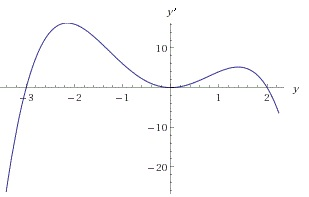
\includegraphics{Plot.jpeg}
\end{center}


\newpage

\section{Lecture 6 on June 3}

1. Motivation: recall how we dealt with linear ODE. Want to find a similar way to operate on some special nonlinear functions.\\

2. Exact Equations

2.1. Definition

2.2. Criterion

2.3. Examples of checking exactness:
$$(3x^2y+ 2xy^5+ 5y) + (x^3+ 5x^2y^4+ 5x)y'=0$$
$$(3x^2y+ 2xy^5+ 6y) + (x^3+ 5x^2y^4+ 5x)y'=0$$

2.3. How to recover the solution: 

\begin{enumerate}
\item Check if $M_y = N_x$ to make sure the ODE is exact. \textbf{If it's not, don't you dare to continue!}
\item Integrate $M$ with respect to $x$ (or $N$ with respect to $y$) to get 
$$\Psi(x,y)=\int Mdx + h(y)$$
(or $\Psi(x,y)=\int Ndy + h(x)$)
\item Use $\displaystyle{\frac{\partial \Psi}{\partial y}=N}$ (or $\Psi_x=M$) to determine $h'(y)$ (or $h'(x)$) and thus determine $h(y)$ (or $h(x)$) and thus $\Psi(x,y)$.
\end{enumerate}
2.4. Remarks: 

(1) If the $h'(y)$ is not independent of $x$, that means you messed up somewhere and don't you dare to continue!

(2) When integrate $h'(y)$, we never worry about the constant 

(3) Don't mess up with the coefficients! \\

3. Examples: 

3.1. $(3x^2y+ 2xy^5+ 5y) + (x^3+ 5x^2y^4+ 5x+2\sin 2y)y'=0$\

3.2. $(3y^2e^{x^2+y^3}+x)y' + 2x e^{x^2 + y^3} + y = 0$

3.3. $(9x^2 + y - 1) - (4y-x)y' = 0, y(1) = 0$: Explicit solution\\

4. Integrating factor methods

4.1. Formulate the equation for exactness

4.2. Impose assumptions to find the conditions

4.3. Summary of the formula 

5. Examples 

5.1. $3xy^2+2y^3 + (2x^2y +3xy^2)y'=0$

5.2. $ydx + (2xy-e^{-2y})dy=0$

\newpage
\section*{Homework}

1. Check if each of the following ODEs is exact. If it is, then find the general solution. If it is not, then try to solve it by finding an integrating factor to make an exact ODE. In case you cannot find an integrating factor, show your attempt and leave it on your paper. 

$$\begin{aligned} 
\text{(a) } & 2x+y+(x+2y)y' = 0 \\
\text{(b) } & x^2 y^3 + x(1+y^2)y' = 0\\
\text{(c) } & (x+2)\sin y dx + x\cos y dy = 0\\
\text{(d) } & ye^{xy}\cos 2x -2e^{xy}\sin 2x + 2x + (xe^{xy}\cos 2x-3)y' = 0\\
\end{aligned}
$$~\\


2. Find the solution to the the IVP 
$$2x-y + (2y-x)y' = 0, y(1) = 3$$
and \textit{approximately} determine the interval of existence. 


\newpage

\section{Lecture 6 on June 4: Numerical Methods}


1. Euler's method

1.1. Idea of Euler's method

1.2. Recurrence relation

1.3. Examples
$$y' = x - y + 1$$

1.4. Error analysis. \\

2. Improved Euler's method

2.1. Idea

2.2. Recurrence relation

2.3. Examples

2.4. Mention the error being proportional to $h^2$\\

3. Runge-Kutta's method

3.1. Idea

3.2. Recurrence Relation

3.3. Examples

3.4. Mention the error being proportional to $h^4$


\newpage

\section*{Homework}

1. Use Euler's method, Improved Euler's method and Runge-Kutta method to find the approximation of $y(3)$ for the following IVP
$$y' = x + y, y(1) = 2$$
using step size $h=1$ and $h=0.5$. You are allowed to use Maple for this problem. 

2. Use concavity method to tell if the approximation obtained by Euler is larger or smaller than the actual solution. 

3. Solve this IVP (use the formula of first order linear ODE) and compute $y(3)$ to see the actual error. 

\newpage

\section{Lecture 9 on June 9th}

0. Announce the second chance club. 

1. Standard form of second order linear ODE, Homogeneous and non-homogeneous. 

2. General theory 

2.1. Existence and uniqueness theorem

Remark: Standard form! 

Remark: In case there's a regular singular point, one may find a special type of series solution (covered in the book from 5.4 to 5.6). However it is way beyond our class. 

Examples: $$\begin{aligned}
1. & t^2 y'' - 2t y' - 4y = 0, y(1)=2, y'(1) = 3 \\
2. & y'' - \tan t y' + t^3y = 0, y(0)=1, y'(0)=3 \\
\end{aligned}$$  

2.2. Principle of superposition with Wronskian: If $y_1, y_2$ are two solutions to the ODE 
$$y'' + p(t)y'+ q(t) y = 0$$
then for ANY numbers $C_1, C_2$, the function $C_1y_1 + C_2y_2$ would also be a solution. 

Example: for $y''- 2y' - 3y = 0$, we know $e^{3t}$ and $e^{-t}$ are solutions. Verify that $2e^{3t}- e^{-t}$ are also solutions. (You can compute by usual methods, but also can be computed in a way that can be generalized to a proof). 

2.3. Moreover, if $y_1$ and $y_2$ are linearly independent functions, then all solutions are of the form $c_1y_1 + c_2y_2$. In other words, 
$$y(t)=C_1y_1(t)+C_2y_2(t)$$
is the general solution to the ODE. 

Example:
$$\begin{aligned}
1. & y_1 = t^2, y_2 = t^3.\\
2. & y_1 = e^{3t}, y_2 = 5 e^{3t}\\
3. & y_1 = e^t, y_2 = 4e^{2t}\\
\end{aligned}$$

2. Second order linear homogeneous ODEs with constant coefficients:
$$ay'' + by' + cy = 0$$
We try $y = e^{rt}$, to get 
$$ar^2 + br + c=0$$
In other words, if $y=e^{rt}$ is a solution to the ODE, then $r$ must satisfy the equation $ar^2+br+c=0$

This equation has three cases:

Case 1: If we managed to solve two distinct real roots $r_1, r_2$, then since $e^{r_1t}$ and $e^{r_2t}$ are automatically linearly independent, we have the general solution
$$y=C_1e^{r_1t} + C_2 e^{r_2 t}$$

Basically quadratic formula works in all the cases

Examples:
$$\begin{aligned}
&y'' - 2y' - 3y = 0 & \text{Previous Example}\\
&y'' - 5y' + 6y = 0 & \text{Factorization Wrong}\\
&2y'' + 7y' + 3y = 0 &\text{Tricky Factorization}\\
&y'' - 4y' - 6y = 0 &\text{quadratic formula}
\end{aligned}$$

Case 2 and Case 3: Tomorrow. 

\newpage
\section*{Homework}

1. Find the interval of existence for the following IVPs
$$\begin{aligned}
\text{(a) }& t^2 y'' + ty' + 6y = 0, y(-1) = 2, y'(-1)=3\\
\text{(b) }& y'' - \cot t y' + (\ln t)y = e^{5t}, y(1)=0, y'(1) = 2\\
\end{aligned}$$

2. Find out if the following functions are linear dependent or independent
$$\begin{aligned}
\text{(a) }& y_1 = e^{2t}\sin t, y_2 = e^{2t}\cos t\\
\text{(b) }& y_1 = e^{3t}, y_2= te^{3t}\\
\end{aligned}$$

3. Find the general solution to the following ODEs
$$\begin{aligned}
\text{(a) }& y'' - 7y' + 12y = 0\\
\text{(b) }& y'' - 5y' - 6y = 0\\
\text{(c) }& y'' + 10y' + 23y = 0\\
\end{aligned}$$

4. Find the solution to the following IVP and determine the long term behavior. (Hint: look at where the limit goes)
$$\begin{aligned}
\text{(a) }& y'' - 25y = 0, y(0)=3, y'(0)=-9\\
\text{(b) }& y'' - y' = 0, y(0)=3, y'(0) =2\\
\text{(c) }& 6y'' + 5y' - 4y = 0, y(0)=0, y'(0) = 0\\
\end{aligned}$$

\newpage

\section{Lecture 10 on June 10}

1. Complex numbers

1.1. Multiplications

Example: $(1+i)(2-i)$, $i(3+i)$, $(cos \theta + i \sin \theta)(1-2i)$

1.2. Geometric Interpretation

1.3. Euler's formula

Example: $e^{\pi/6 i}$, $r^4 + 1 = 0$

1.4. Taking fourth roots

Example: $(-1)^{1/4}$, $2^{1/3}$. \\


2. Second order linear homogeneous ODE with constant coefficients: continued

2.1. Recall: characteristic equation, characteristic root. 

2.2. Recall: distinct real roots \\

3. Complex root case

3.1. Formula: $C_1 e^{\alpha t}\cos \beta t + C_2 e^{\alpha t}\sin \beta t$

Examples: $y'' + y = 0$, $y'' + 2y' + 8y = 0$, $y'' - y' + y = 0$

3.2. Formulation of complex solutions.

3.3. Getting real solutions. 

3.4. Graphs and Long term behaviors (growing, steady, decaying)

4. Repeated Root Case

4.1. Formula 

Examples: $y'' - 2y' + y = 0$, $4y'' - 4y' + y = 0$

4.2. Idea of Variation of parameter

4.3. Reduction of Order

4.4. Long term behaviors (eventually positive, eventually negative)

\newpage

\section*{Homework}

1. Find the general solutions to the following ODEs

$$\begin{aligned}
\text{(a)  }& y'' - 2y' + 2y = 0\\
\text{(b)  }& y'' + 2y' + 2y = 0\\
\text{(c)  }& y'' + 25 y = 0\\
\text{(d)  }& 4y'' + 16 y' + 25y = 0\\
\text{(e)  }& 4y'' - 20 y' + 25y = 0\\
\text{(f)  }& y'' - 6y' + 9y = 0\\
\end{aligned}$$

2. Find the solutions to the following IVPs and state if the solution is growing, steady or decaying

$$\begin{aligned}
\text{(a)  }& y'' + 4y = 0, y(0)=0, y'(0) = 1\\
\text{(b)  }& y'' - 4y' + 5y = 0, y(0) = 3, y'(0)=0\\
\text{(c)  }& y'' + 4y' + 5y = 0, y(0) = 3, y'(0)=0\\
\end{aligned}$$

3. Find the solutions to the following parameterized IVPs and determine the critical value of $\alpha$ when the long term behavior changes
$$\begin{aligned}
\text{(a)  }& y'' - 3y' - 4y = 0, y(0)=\alpha, y'(0) = 2\\
\text{(b)  }& y'' - 4y' + 4y = 0, y(0)=1, y'(0) =\alpha\\
\end{aligned}$$

\newpage
\section{Lecture 11 on June 11}

0. Reduction of Order

0.1. Variation of Parameter

0.2. Application to the first order differential equation

0.3. Application to second order homogeneous ODE

Examples: $y'' - 2ry' + r^2 y = 0, y_1 = e^{rt}$, $ty'' - y' - 4t^3 y = 0, y_1 = \sin t^2$. \\

1. Free Vibration

1.1. Physics background and equation of motion: A mass is attached with a spring vertically. Let $u$ be \underline{the displacement of the mass FROM THE EQUILIBRIUM} (which characterizes how the mass is stretched ``further'' from where it stays still). Then the equation of motion in general looks like
$$m u'' + \gamma u' + k u = 0$$
where $m$ stands for the \underline{mass}, $\gamma$ represent the \underline{damping}, $k$ is the \underline{spring constant}.

1.2. Undamped Case: Natural Frequency, Amplitude and Phase

Example: Suppose that a mass weighing 10 lb stretches a spring 2 in. If the mass is displaced an additional 2 in and is then set in motion with an initial upward velocity of 1 ft/s, determine the position
of the mass at any later time. Also determine the period, amplitude, and phase of the motion.

1.3. Underdamped Case: $\gamma<\sqrt{4km}$. Quasi-frequency, Quasi-Period. 

Example: A mass weighing 4 lb stretches a spring 2 in. Suppose that the mass is given an additional 6 in displacement in the positive direction and then released. The mass is in a medium that exerts a viscous resistance of 6 lb when the mass has a velocity of 3 ft/s. Formulate the IVP and solve it. 

1.4. Overdamped Case: $\gamma > \sqrt{4km}$

Example: A mass weighing 4 lb stretches a spring 1.5 in. The mass is in a medium that exerts a viscous resistance of 15 lb when the mass has a velocity of 3 ft/s. Suppose the mass is given an additional 6 in displacement. Find out the condition for the velocity such that the mass passes through the equilibrium (overshoot). 

Added June 15th: In class I actually used the following data: A mass weighing 4lb stretches a spring 2 in. 


1.5. Critically Damped Case: $\gamma = \sqrt{4km}$

Example: A mass weighing 4 lb stretches a spring 1.5 in. Suppose that the mass is given an additional 6 in displacement in the positive direction and then released. The mass is in a medium that exerts a viscous resistance of 12 lb when the mass has a velocity of 3 ft/s. Formulate the IVP and solve it


\newpage

\section*{Homework}

1. Knowing that $y_1$ is a solution to the following given homogeneous ODEs, find the general solution to the ODE:
$$
\begin{aligned}
\text{(a)  }& y_1 = \frac 1 t, t^2 y'' + 3t y' + y = 0\\
\text{(b)  }& y_1 = e^t, (t-1)y'' - ty' + y = 0\\
\end{aligned}
$$

2. A mass weighing 2 lb stretches a spring 6 in. If the mass is pulled down an additional 3 in
and then released, and if there is no damping, determine the position $u$ of the mass at any
time $t$. Find the frequency, period, and amplitude of the motion.

3. With all the data as in Problem 2 and in addition assume there is damping. Find out the condition of the damping coefficient such that the vibration is underdamped, critically damped, and overdamped. 

4. With all the data as in Problem 2 and in addition assume the vibration is critically damped, find out the condition on the velocity such that overshoot happens. 

5. Maple Lab 3 is assigned and is due the Monday after the next. 

\newpage

\section{Lecture 12 on June 15th}

0. Leftovers from the previous class. \\

1. Euler's equation.

1.1. Definition

1.2. Interval of Existence. 

1.3. Characteristic Equation 

1.4. Formula for the general solution

The time is probably not enough cover the case for the general solution for $t<0$ case. Just mention the case of $t>0$ and leave an exercise discussing generalizations. 

Examples: $t^2y'' + 4t y' + 2y = 0$, $t^2 y'' - 3t y' + 4y=0, t^2 y'' + 3t y' + 5y = 0$\\

2. How comes the formula

2.1. Real distinct characteristic roots.

2.2. Complex characteristic roots.

2.3. Repeated Roots. Application of Variation of Parameter.\\

3. Issues in generalization to $t<0$ case

3.1. General solution is indeed easy. 

3.2. The derivative issues.

Example: $t^2y'' - ty' +y = 0, y(-1)=1, y'(-1)=2$

\newpage

\section*{Homework}

0. Problem 3, 4, 5 in HW 11. 

1. Find the general solution to the following ODEs

$$\begin{aligned}
\text{(a)  }&2x^2 y'' - 4x y' + 6y = 0\\
\text{(b)  }&x^2 y'' - 5xy' + 9y = 0\\
\text{(c)  }&(x+1)^2 y'' + 3(x+1)y' + 0.75y = 0\\
\end{aligned}$$


2. Find the solution to the following IVPs

$$\begin{aligned}
\text{(a)  }&2x^2 y'' + xy' - 3y = 0, y(1) = 1, y'(1) = 4\\
\text{(b)  }&4x^2 y'' + 8xy' + 17y = 0, y(1) = 2, y'(1) = -3\\
\end{aligned}
$$

3. (Bonus) Prove that if the characteristic roots of a second order linear homogeneous ODE are real, then the solution passes through the equilibrium at most once. Use this fact to argue that in the critically damped case or in the overdamped case, the mass will pass through the equilibrium at most once. 

Solution: 
1. 
$$
\begin{aligned}
\text{(a)  }& y = C_1 x^{3/2} \cos (\frac {\sqrt 3}{2}\ln x) + C_2 x^{3/2} \sin (\frac {\sqrt 3}{2}\ln x)\\
\text{(b)  }& y = C_1 x^3 + C_2 x^3 \ln x\\
\text{(c)  }& y = C_1 (x+1)^{-1/2} + C_2 (x+1)^{-3/2}\\
\end{aligned}
$$


2. 
$$
\begin{aligned}
\text{(a)  }&y = 2x^{3/2} - x^{-1}\\
\text{(b)  }&y = 2x^{-1/2}\cos(2\ln x) - x^{-1/2}\sin(2\ln x)
\end{aligned}
$$

\newpage
\section{Lecture 13 on June 16}

1. General Theory of nonhomogeneous linear ODE

1.1. Proposition: If $Y_1$ and $Y_2$ are two solutions to 
$$y'' + p(t) y' + q(t)y = g(t)$$
then $Y_1 - Y_2$ will be a solution of 
$$y'' + p(t) y' + q(t)y = 0$$

1.2. Once we know a particular solution $Y$, then we know that
$$C_1 y_1 + C_2 y_2 + Y$$ will be a solution for any number $C_1$ and $C_2$. 

1.3. By the existence and uniqueness theorem, for any second order linear ODE, there will be at most two arbitrary constants. Therefore the above expression actually gives the general solution.

1.4. $C_1y_1 + C_2 y_2$ is referred as complementary solution. $Y$ is referred as particular solution.\\

2. Application to second order linear ODE with constant coefficients

Use the recitation notes on Mar. 8, 2015

\newpage 

\section*{Homework}

1. Find the general solution to the following ODEs

$$\begin{aligned}
\text{(a)  }&  y'' + 2y' + y = 5\\
\text{(b)  }&  y'' - 5y' + 6y = t+6  \\
\text{(c)  }&  y'' - 5y' + 6y = te^t\\
\text{(d)  }&  y'' + y = e^t\\
\text{(e)  }&  y'' + y = 3\sin 2t + 6 \cos 2t  \\
\end{aligned}$$

2. Find the general solution to the following ODEs. 
$$\begin{aligned}
\text{(a)  }&  y'' - 5y' + 6y = e^{3t}\\
\text{(b)  }&  y'' + y = \sin t \\
\text{(c)  }&  y'' + 2y' + y = te^{-t}\\
\text{(d)  }&  y'' + 2y' - 3y = e^{-3t} + \sin 2t
\end{aligned}$$

3. Let $\omega_0$ be a constant real number and let $\omega$ be another constant real number with $\omega \neq \omega_0$. Solve the following IVPs
$$\begin{aligned}
\text{(a)  }&  y'' + \omega_0^2 y = \cos \omega t, y(0)=0, y'(0) = 0\\
\text{(b)  }&  y'' + \omega_0^2 y = \cos \omega_0 t, y(0)=0, y'(0) = 0\\
\end{aligned}$$

Solutions:

1. 
$$
\begin{aligned}
\text{(a)  }&  y= C_1 e^{-t} + C_2 e^{-t}+5\\
\text{(b)  }&  y= C_1 e^{2t}+ C_2e^{3t} + \frac 1 6 t + \frac{41}{36} \\
\text{(c)  }&  y =C_1 e^{2t}+ C_2 e^{3t} + (\frac 1 2 t+\frac 3 4)e^t\\
\text{(d)  }&  y = C_1 \cos t + C_2 \sin t + \frac 1 2 e^t\\
\text{(e)  }&  y = C_1 \cos t + C_2 \sin t - \sin 2t - 2 \cos 2t \\
\end{aligned}
$$

2. 
$$\begin{aligned}
\text{(a)  }&  y = C_1 e^{3t}+ C_2 e^{2t}+ te^t\\
\text{(b)  }&  y = C_1 \cos t + C_2 \sin t - \frac 1 2 t\cos t \\
\text{(c)  }&  y = C_1 e^{-t} + C_2 te^{-t} - \frac 1 6 t^3 e^{-t}\\
\text{(d)  }&  y = C_1 e^{t} + C_2 e^{-3t} - \frac 1 4 te^{-3t} - \frac 7 {65} \sin 2t -\frac 4 {65}\cos 2t
\end{aligned}$$

3. 
$$
\begin{aligned}
\text{(a)  }&  y = \frac 1 {\omega^2-\omega_0^2} \left(\cos(\omega_0 t) -\cos(\omega t)\right)\\
\text{(b)  }&  y = \frac 1 {2\omega_0}t\sin \omega_0 t\\
\end{aligned}
$$

\newpage
\section{Lecture 15 on June 18, 2015}

0. Leftovers

0.1. First try template independent of left hand side

0.2. Failure of first try template,  modification, determining the correct template without trying. Use recitation notes.\\

1. Variation of parameters.

Idea: Varying the parameters in the complementary solution. 

1.1. Deduction of the equation: For the ODE
$$y'' + p(t)y' + q(t)y = g(t)$$
Let $C_1y_1 + C_2y_2$ be the complementary solution. Set $Y = u_1y_1 + u_2y_2$, we first compute $Y'$
$$\begin{aligned}
Y' &= u_1' y_1 + u_1y_1' + u_2' y_2 + u_2 y_2' 
\end{aligned}$$
For simplicity, we set $u_1'y_1+u_2'y_2$ to be zero, so we don't have to deal with second derivatives of $u_1$ and $u_2$. Thereby
$$\begin{aligned}
Y' &= u_1y_1' + u_2y_2' \\
Y''&= u_1'y_1' + u_1y_1'' + u_2'y_2' + u_2y_2'' \\
Y'' + pY' + q Y &= u_1y_1' + u_1y_1'' + u_2y_2' + u_2y_2'' + p(u_1y_1' + u_2y_2') + q(u_1y_1 + u_2y_2) \\
&= u_1(y_1'' + py_1' + qy_1) + u_2(y_2'' + py_2' + qy_2) + u_1'y_1' + u_2'y_2'\\
&= u_1'y_1' + u_2'y_2'
\end{aligned}$$
Setting it equal to $g$ and together with the assumption we have
$$\left\{\begin{aligned}
y_1u_1' + y_2u_2' = 0\\
y_1'u_1'+y_2'u_2' = g(t)
\end{aligned}\right.$$

1.2. Deduction of the integration formula.

1.2.1. Remark: Cramer's rule

1.3. Remark: $g(t)$ must come from the standard form! \\

2. Examples

2.1. Find the general solutions to 
$$y'' - 2y' + y = \frac{e^t}{1+t^2}$$
$$x^2 y'' - 3x y' + 4y = x^2 \ln x$$

2.2. Knowing that $y_1 = e^t$ is a solution to the ODE
$$ty'' - (1+t)y' + y = 0$$
Find the general solution to
$$ty'' - (1+t)y' + y = t^2 e^{2t}$$
 

3. Forced Undamped Vibrations. Natural frequency $\omega_0$. External Frequency $\omega$

3.1. $\omega \neq \omega_0$. General solution. Beats. 

3.2. $\omega = \omega_0$. General solution. Resonance. 

Example: Suppose that a mass weighing 4 lb stretches a spring 1.5 in. Assume there is no damping. Also the mass is subject to an external force as strong as $2\cos \omega t$ lb. At $t=0$, the mass is displaced an additional 2 in and is then set in motion with an initial upward velocity of 1 ft/s. Determine the frequency of the external force for resonance to happen and then the position of the mass at any later time. 

4. Forced Damped Vibration.

4.1. General solution

4.2. Transient solution, Steady-State solution.

Example: Suppose that a mass weighing 4 lb stretches a spring 1.5 in. The mass is in a medium that exerts a viscous resistance of 15 lb when the mass has a velocity of 3 ft/s. Also the mass is subject to an external force as strong as $2\cos 16 t$ lb. At $t=0$, the mass is displaced an additional 2 in and is then set in motion with an initial upward velocity of 1 ft/s. 

\newpage
\section*{Homework}

1. A mass weighing 2 lb stretches a spring 6 in. Assuming there's no damping in the system. If the mass is pulled down an additional 3 in and then released, meanwhile is acted on by an additional oscillating force with amplitude 1 lb and phase 0. Find out the frequency of the force such that resonance happen, and determine the position at any time $t$ by solving the system. 

2. With all the data as above, suppose for now the system is subject to a damping force that is as strong as 2 lb when the velocity of the mass is 4 ft/s. Find the transient solution and the steady-state solution. 

3. Find the general solution to the following ODEs
$$
\begin{aligned}
\text{(a)  } & y'' + y = \tan t\\
\text{(b)  } & 4y'' + y = 2 \sec(t/2)\\
\text{(c)  } & x^2 y'' - 2y = 3x^2 - 1, x>0\\
\end{aligned}
$$

4. Knowing $y_1$ is a solution to the homogeneous ODE, find the general solution to the following ODEs
$$
\begin{aligned}
\text{(a)  } & y_1 = x, x^2 y'' - x(x+2)y' + (x+2) y(x) = 2x^2, x>0\\
\text{(b)  } & y_1 = e^x, (1-x)y'' + xy' - y = 2(1-x)\\
\end{aligned}
$$

5. (Bonus) Apply the variation of parameters to the first order linear ODE
$$y' + p(t) y = g(t)$$
to obtain the formula of the general solution. 
(Hint: Solve the homogeneous ODE $y' + p(t)y = 0$ first to get the complementary solution $Cy_1$. Then set $Y(t)=u(t)y_1(t)$ and put in the ODE to find $Y$. So the general solution would then be $Cy_1 + Y$. 

Solutions:

1. $\omega = 8$. Solution: $u = 0.25 \cos 8t + t \sin 8t$

2. $u(t) = C_1 e^{-4t}\cos 4\sqrt 3 t + C_2 e^{-4t} \sin 4\sqrt 3 t + \frac 1 4 \sin 8t$. 

3. 
$$
\begin{aligned}
\text{(a)  } & y = C_1 \cos t + C_2 \sin t - \ln|\sec t + \tan t| \cos t\\
\text{(b)  } & y = C_1 \cos \frac t 2 + C_2 \sin \frac t 2 + t\sin \frac t 2 + 2\cos \frac t 2 \ln|\cos frac t 2|\\
\text{(c)  } & y = C_1 x^2 + C_2 \frac 1 x + \frac 1 2 + x^2 \ln x. \\
\end{aligned}
$$

4. 
$$
\begin{aligned}
\text{(a)  } & y = C_1 x + C_2 xe^x - 2x\ln x - 2xe^{x} \int \frac 1 {xe^x}dx\\
\text{(b)  } & y = C_1 x + C_2 e^x - 2x \ln(x-1) + e^x \int \frac{2x}{(x-1)e^x}dx \\
\end{aligned}
$$
\newpage 
\section{Lecture 17 on June 23, 2015}


0. General Theory

Homogeneous ODE

0.1. Fundamental Set of Solutions: $y_1, \cdots, y_n$ that are linearly independent. In other words, $W(y_1, \cdots, y_n)\neq 0$

0.2. Principle of Superposition: If the fundamental set of solutions consists of functions $y_1, \cdots, y_n$, then the general solution is $C_1y_1 + C_2 y_2 + \cdots C_n y_n$

Nonhomogeneous ODE

0.3. Structure of Solution: $y= y_c + Y$. 

0.4. Principle of Superposition: If $Y_1$ is a particular solution to 
$$a_ny^{(n)} + a_{n-1}y^{(n-1)} + \cdots + a_1 y' + a_0 = g_1(t)$$
and $Y_2$ is a particular solution to
$$a_ny^{(n)} + a_{n-1}y^{(n-1)} + \cdots + a_1 y' + a_0 = g_2(t)$$
then $Y_1+Y_2$ is a particular solution to 
$$a_ny^{(n)} + a_{n-1}y^{(n-1)} + \cdots + a_1 y' + a_0 = g_1(t)+g_2(t)$$
\ \\


1. Higher order linear homogeneous ODEs with constant coefficients. 
$$a_ny^{(n)} + a_{n-1}y^{(n-1)} + \cdots + a_1 y' + a_0 = 0$$


1.2. Characteristic Equation. 

1.3. Theorem: Every real polynomial can be factorized to products of linear polynomials and quadratic polynomial. Meaning: real roots or imaginary roots. 

1.4. If $r$ is a real single root, then it contributes to one function in the fundamental set of solutions
$$e^{rt}$$

1.5. If $r$ is a real root repeated $m$ times, then it contributes to the following $m$ functions in the fundamental set of solutions
$$e^{rt}, te^{rt}, \cdots, t^{m-1}e^{rt}$$

1.6. If $r=\alpha + i\beta$ is a complex root repeated $m$ times, we know from algebra that the root $\overline{r} = \alpha-i\beta$ should also be repeated $m$ times. They contributes to $2m$ functions in the fundamental set of solutions
$$e^{\alpha t}\cos \beta t, e^{\alpha t}\sin \beta t, te^{\alpha t}\cos \beta t, te^{\alpha t}\sin \beta t, \cdots, t^{m-1}e^{\alpha t}\cos \beta t, t^{m-1}e^{\alpha t}\sin \beta t$$

Examples: 

Distinct Real roots: $y''' - y' = 0$

Distinct and Repeated Real roots $y''' - y'' - y' + y = 0$

Repeated Real roots: $y'''-3y''+3y'-y=0$

Complex Roots: $y''' - y = 0$

Real and Complex Roots: $y''' - y'' + y' - y = 0$

Repeated Complex Roots: $y^{(4)} + 8y'' + 16 y = 0$\\

2. Higher order linear nonhomogeneous ODE with constant coefficients
$$a_n y^{(n)} + a_{n-1}y^{(n-1)}+ \cdots + a_1 y' + a_0 y = g(t)$$


2.1. Method of Undetermined Coefficients

Example: $y''' - y'' - y' + y = 8e^t + 4e^{-t} + 25\cos 2t + t^2 $

General solution
$$y(t)=y_c(t)+Y(t)=C_1e^t + C_2 te^t + C_3 e^{-t}+2t^2 e^t+  te^{-t} + t^2 + 2t + 4 + \cos 2t - 2\sin 2t$$

2.2. Determining the final template

Examples: Review Questions 2 in Spring 2014

\newpage
\section*{Homework}

1. Find the general solutions the following ODEs
$$
\begin{aligned}
\text{(a)  }& y''' - y'' - y' + y = 2e^{-t} + 3\\
\text{(b)  }& y^{(4)} - y = 3t + \cos t\\
\text{(c)  }& y''' + y'' + y' + y = e^{-t} + 4t\\
\text{(d)  }& y''' - y' = 2 \sin t\\
\text{(e)  }& y^{(4)} - 4y = t^2 + e^t\\
\text{(f)  }& y^{(4)} + 2y'' + y = 3 + \cos 2t\\
\text{(g)  }& y^{(6)} + y''' = t \\
\text{(h)  }& y^{(4)} + y''' = \sin 2t\\
\end{aligned}
$$

2. Determine the final template of the particular solution for the following ODEs and use Maple to solve it. 

$$
\begin{aligned}
\text{(a)  }& y''' - 2y'' + y' = t^3 + 2e^t\\
\text{(b)  }& y''' - y' = te^{-t} + 2 \cos t\\
\text{(c)  }& y^{(4)} - 2y'' + y = e^t + \sin t\\
\text{(d)  }& y^{(4)} + 4y'' = \sin 2t + te^t + 4\\
\text{(e)  }& y^{(4)} - y''' - y'' + y' = t^2 + 4 + t \sin t\\
\text{(f)  }& y^{(4)} + 2y''' + 2y'' = 3e^t + 2te^{−t} + e^{−t} sin t\\
\end{aligned}
$$

Solution: 
1. 
$$
\begin{aligned}
\text{(a)  }& y = C_1 e^t + C_2 te^t + C_3 e^{-t} + \frac 1 2 te^{-t}+ 3\\
\text{(b)  }& y = C_1 e^t + C_2 e^{-t} + C_3 \cos t + C_4 \sin t - 3t - \frac 1 4 t\sin t\\
\text{(c)  }& y = C_1 e^{-t} + C_2 \cos t + C_3 \sin t _+ \frac 1 2 te^{-t} + 4t - 4\\
\text{(d)  }& y = C_1 + C_2 e^t + C_3 e^{-t} + \cos t\\
\text{(e)  }& y = C_1 + C_2 t + C_3 e^{-2t} + C_4 e^{2t} - \frac 1 3 e^t - \frac 1 {48}t^4 - \frac 1 6 t^2\\
\text{(f)  }& y = C_1 \cos t + C_2 \sin t + C_3 t \cos t + C_4 t\sin t + 3 + \frac 1 9 \cos 2t\\
\text{(g)  }& y = C_1 + C_2 t + C_3 t^2 + C_4 e^{-t} + C_5 e^{-t/2}\cos \frac{\sqrt 3}2t + C_6 e^{-t/2} \sin \frac{\sqrt 3} 2 t + \frac 1 24 t^4 \\
\text{(h)  }& y = C_1 + C_2 t + C_3 t^2 + C_4 e^{-t} + \frac 1 {20}\sin 2t + \frac 1 {40}\cos 2t\\
\end{aligned}
$$
2. 
$$
\begin{aligned}
\text{(a)  }& Y = t(At^3 + Bt^2 + Ct + D) + Bt^2 e^t\\
\text{(b)  }& Y = t(At+B)e^{-t} + B\cos t + C\sin t\\
\text{(c)  }& Y = At^2 e^t + B\cos t + C\sin t\\
\text{(d)  }& Y = At^2 + (Bt+C) e^t + t(D\cos 2t + E\sin 2t)\\
\text{(e)  }& Y = t(At^2 + Bt+ C)+ (Dt+E)\cos t + (Ft+G) \sin t\\
\text{(f)  }& Y = Ae^t + (Bt+C)e^{-t} + t(De^{-t}\cos t + Ee^{-t}\sin t)\\
\end{aligned}
$$

\newpage
\section{Lecture 19 on June 28, 2015}

1. Review of power series

1.1. A power series centered at a point $x_0$ is an infinite series of the form
$$\sum_{n=0}^\infty a_n (x-x_0)^n$$

1.2. Radius of convergence: if $|x-x_0|<r$ then the series converges, if $|x-x_0|>r$ then the series diverges, if $|x-x_0|=r$ we can't tell in general. 

1.3. $R = \lim_{n\to \infty} \left|\frac {a_n}{a_{n+1}}\right|$

1.4. Why study power series:

1.4.1. Near every point, every elementary function (exp, log, trig., inverse trig.) admits a series expansion, by Taylor's theorem.

1.4.2. There are a lot more functions that cannot be expressed as elementary functions, yet can be expressed as power series. Example: $\int_{-\infty}^x e^{-x^2}$. 

1.4.3. In general one can ALWAYS find series solutions, if the coefficients satisfies certain regularity. 

2. Dr. Gross's Video Lecture

3. More Examples: $(2+x^2)y'' - xy' + 4y = 0$, $e^xy''+ xy = 0$

\newpage

\section*{Homework}

1. Find the first four terms in each of two solutions $y_1$ and $y_2$ (unless the series terminates
sooner) about the given point $x_0$.

$$
\begin{aligned}
\text{(a)  }& y'' - xy' - y = 0, x_0 = 1\\
\text{(b)  }& y'' - xy' - y = 0, x_0 = 0\\
\text{(c)  }& y'' + xy' + 2y = 0, x_0 = 0\\
\text{(d)  }& x^2 y'' - x(x+2)y' + (x+2)y = 0, x_0 = 0\\
\text{(e)  }& (3-x^2) y'' - 3x y' - y = 0, x_0 = 0\\
\end{aligned}
$$

Added 12:15PM: Problem 1d is set to be a bonus problem. It can still be solved using the techniques we talked about in class but just accidentally, due to the reason that $x_0$ is indeed a singular point (which does not belong to our current syllabus). Also Problem 1e was changed due to the same reason. Also in Problem 1d, the recurrence relation is indeed tricky to solve. 

2. Determine a lower bound for the radius of convergence of series solutions about each given point $x_0$ for the given differential equation.
$$
\begin{aligned}
\text{(a)  }&y'' + 4y' + 6xy = 0; x_0 = 0, x_0 = 4\\
\text{(b)  }& (x^2 - 2x - 3)y'' + xy + 4y = 0; x_0 = 4, x_0 = -4, x_0 = 0\\
\text{(c)  }& (1 + x^3)y'' + 4xy' + y = 0; x_0 = 0, x_0 = 2\\
\text{(d)  }& xy'' + y = 0; x_0 = 1
\end{aligned}
$$

Solutions:
1. 
$$
\begin{aligned}
\text{(a)  }& y = a_0 \left(1 + \frac 1 2 (x-1)^2 + \frac 1 6 (x-1)^3 + \frac 1 6 (x-1)^4 + \cdots\right) \\
& + a_1 \left((x-1) + \frac 1 2(x-1)^2 +\frac 1 2(x-1)^3 +\frac 1 4(x-1)^4+\cdots \right)\\
\text{(b)  }& y = a_0 \left(1 + \frac {x^2} 2 + \frac{x^4}{8} + \frac {x^6}{48}+\cdots\right) + a_1 \left(x + \frac{x^3}{3} + \frac{x^5}{15} + \frac{x^7}{105}+ \cdots\right)\\
\text{(c)  }& y = a_0 \left(1 - x^2 + \frac 1 3 x^4 - \frac 1 {15} x^6+\cdots\right)+a_1\left( x - \frac 1 2 x^3 + \frac 1 8 x^5 -\frac 1 {48}x^7 + \cdots\right)\\
\text{(d)  }& y = a_1 x + a_2 \left(x^2 + \frac 1 2 x^3 + \frac 1 6 x^4 + \frac 1 {24}x^5 + \cdots\right)\\
\text{(e)  }& y = a_0 \left(1 + \frac 1 6 x^2 + \frac 1 {24} x^4 + \frac 5{432}x^6 + \cdots\right)+a_1\left(x + \frac 2 9 x^3 + \frac 8 {135}x^5 + \frac{16}{945}x^7 + \cdots\right)\\
\end{aligned}
$$

2. 
$$
\begin{aligned}
\text{(a)  }& x_0 = 0, R = \infty; x_0 = 4, R = \infty\\
\text{(b)  }& x_0 = 0, R \geq 1; x_0 = 4, R \geq 1; x_0 = -4, R \geq 3\\
\text{(c)  }& x_0 = 0, R \geq 1; x_0 = 2, R\geq 1\\
\text{(d)  }& x_0 = 1, R \geq 1
\end{aligned}
$$


\newpage
\section{Lecture 22 on July 1, 2015}

1. Multiplications

2. Linear Equations in terms of matrices

3. Linear dependence and independence

4. Eigenvalues and Eigenvectors

\newpage

\section*{Homework}

1. Solve the following linear systems of equations
$$\begin{aligned}
\text{(a)  }&  \left\{\begin{array}{rcl}
x_1 - x_2 + x_3 &=&2 \\
2x_1 - x_2 - x_3 &=& 2 \\
-x_1 - 3x_2 + x_3 &=& -4 \\
\end{array}\right.\\
\text{(b)  }&  \left\{\begin{array}{rcl}
x_1 - x_2 + x_3 &=&1 \\
2x_1 - x_2 - x_3 &=& 0 \\
5x_1 - 3x_2 - x_3 &=& 2 \\
\end{array}\right.\\
\text{(c)  }&  \left\{\begin{array}{rcl}
x_1 - x_2 + x_3 &=&1 \\
2x_1 - x_2 - x_3 &=& 0 \\
5x_1 - 3x_2 - x_3 &=& 1 \\
\end{array}\right.\\
\text{(d)  }&  \left\{\begin{array}{rcl}
x_1 - x_2 + x_3 &=&1 \\
2x_1 - 2x_2 +2 x_3 &=& 2 \\
-5x_1 + 5x_2 - 5x_3 &=&-5 \\
\end{array}\right.\\
\end{aligned}$$

2. Determine whether the members of the given set of vectors
are linearly independent. If they are linearly dependent, find a linear relation among them. 
$$\begin{aligned}
\text{(a)  }& \overrightarrow{v_1} = \left[\begin{array}{c}
1\\ 1 \\0 
\end{array}\right], \overrightarrow{v_2} = \left[\begin{array}{c}
1\\ 0 \\1 
\end{array}\right], \overrightarrow{v_3} = \left[\begin{array}{c}
0\\ 1 \\1 
\end{array}\right]. \\
\text{(b)  }& \overrightarrow{v_1} = \left[\begin{array}{c}
2\\ 1 \\0 
\end{array}\right], \overrightarrow{v_2} = \left[\begin{array}{c}
0\\ 1 \\0 
\end{array}\right], \overrightarrow{v_3} = \left[\begin{array}{c}
-1\\ 2 \\0 
\end{array}\right]. \\
\text{(c)  }& \overrightarrow{v_1} = \left[\begin{array}{c}
1\\ 2 \\-1 
\end{array}\right], \overrightarrow{v_2} = \left[\begin{array}{c}
2\\ 1 \\1 
\end{array}\right], \overrightarrow{v_3} = \left[\begin{array}{c}
1\\ -1 \\2 
\end{array}\right]. \\
\text{(d)  }& \overrightarrow{v_1} = \left[\begin{array}{c}
1\\ 2 \\-2 
\end{array}\right], \overrightarrow{v_2} = \left[\begin{array}{c}
3\\ 1 \\0 
\end{array}\right], \overrightarrow{v_3} = \left[\begin{array}{c}
2\\ -1 \\1 
\end{array}\right], \overrightarrow{v_4} = \left[\begin{array}{c}
4\\ 3 \\-2 
\end{array}\right]. \\
\end{aligned}$$

3. Find the eigenvalues and eigenvectors of the following matrices
$$\begin{aligned}
\text{(a)  }&  \left[\begin{array}{cc}
5 & -1 \\
3 & 1 
\end{array}\right]\\
\text{(b)  }&   \left[\begin{array}{cc}
2 & -1 \\
5 & 4 
\end{array}\right]\\
\text{(c)  }&   \left[\begin{array}{ccc}
3 & 2 & 4 \\
2 & 0 & 2 \\ 
4 & 2 & 3 
\end{array}\right]\\
\end{aligned}$$

\newpage

\section{Lecture 23 on July 2, 2015}

1. General theory systems of first order linear ODEs
$$\overrightarrow{x}'(t) = A(t) \overrightarrow{x}(t)$$
In $n$-variable case
$$\left\{\begin{array}{c}
x_1'= p_{11}(t) x_1 + \cdots + p_{1n}(t)x_n + g_1(t)\\
x_2'= p_{21}(t) x_1 + \cdots + p_{2n}(t)x_n + g_2(t)\\
\cdots \cdots \cdots \\
x_n'= p_{n1}(t) x_1 + \cdots + p_{nn}(t)x_n + g_n(t)\\
\end{array}\right.$$

Existence and Uniqueness Theorem: If $p_{ij}(t), i,j = 1, ..., n$ and $g_i(t), i=1, ... , n$ are continuous over an interval $(\alpha,\beta)$ that contains $t_0$, then there exists a unique solution to the initial value problem 
$$\left\{\begin{array}{c}
x_1'= p_{11}(t) x_1 + \cdots + p_{1n}(t)x_n + g_1(t)\\
x_2'= p_{21}(t) x_1 + \cdots + p_{2n}(t)x_n + g_2(t)\\
\cdots \cdots \cdots \\
x_n'= p_{n1}(t) x_1 + \cdots + p_{nn}(t)x_n + g_n(t)\\
\end{array}\right., x_1(t_0)=x_1^0, \cdots, x_n(t_0)=x_n^0,$$
over the interval $(\alpha, \beta)$. 

Remark: We'll only focus on the homogeneous system, i.e., the case when all $g_i(t) = 0$. \\

Principle of Superposition: Vector functions $\overrightarrow{x^{(1)}}(t), \cdots, \overrightarrow{x^{(n)}}(t)$ are linearly independent solutions to the system $\overrightarrow{x}'(t) = A(t) x(t)$, then the general solution to the linear homogeneous system is 
$$\overrightarrow{x}(t) = C_1 \overrightarrow{x^{(1)}}(t)+ \cdots+ C_n\overrightarrow{x^{(n)}}(t)$$

Linearly independent means the Wronskian of the vector functions are not constantly zero. \\

Relations to the first order ODE



2. System of Linear ODEs with Constant coefficients:
$$\overrightarrow{x}'(t)=A \overrightarrow{x}(t) $$
Idea: Try $\overrightarrow{x}(t) = e^{\lambda t}\overrightarrow{v}$ to find some solutions. Then use the principle of superposition to solve the problem 

\newpage

\section*{Homework}

\newcommand{\ORA}{\overrightarrow}

Solve the following linear systems

$$\begin{aligned}
\text{(a)  } & \ORA{x}' = 
\left[\begin{array}{rr}
-2 & 1 \\
 1 & -2 \end{array}\right]\ORA{x}\\
\text{(b)  } & \ORA{x}' = 
\left[\begin{array}{rr}
 3 & -2 \\
 2 & -2 \end{array}\right]\ORA{x}\\
\text{(c)  } & \ORA{x}' = 
\left[\begin{array}{rr}
 1 & -2 \\
 3 & 4 \end{array}\right]\ORA{x}\\
\text{(d)  } & \ORA{x}' = 
\left[\begin{array}{rr}
 2 & -1 \\
 3 & -2 \end{array}\right]\ORA{x}\\
\text{(e)  } & \ORA{x}' = 
\left[\begin{array}{rrr}
 1 & 1 & 1\\
 2 & 1 & -1\\
 -8 & -5 & -3\end{array}\right]\ORA{x}\\
\text{(f)  } & \ORA{x}' = 
\left[\begin{array}{rrr}
 1 & -1 & 4\\
 3 & 2 & -1\\
 2 & 1 & -1\end{array}\right]\ORA{x}\\
\end{aligned}$$

\newpage

\section{Lecture 24 on July 6, 2015}

Real, complex and repeated eigenvalue cases. 

Use the old recitation notes. 

\newpage

\section*{Homework}

Solve the following initial value problems:

$$\begin{aligned}
\text{(a)  } & \ORA{x}' = 
\left[\begin{array}{rr}
-4 & 2 \\
-15 & 7 \end{array}\right]\ORA{x}, \ORA{x}(0) = \left[\begin{array}{r}
 2 \\
 0 \end{array}\right]\\
\text{(b)  } & \ORA{x}' = 
\left[\begin{array}{rr}
 3 & -2 \\
 4 & -1 \end{array}\right]\ORA{x}, \ORA{x}(0) = \left[\begin{array}{r}
 1 \\
 1 \end{array}\right]\\
\text{(c)  } & \ORA{x}' = 
\left[\begin{array}{rr}
 -3 & 2 \\
 -1 & -1 \end{array}\right]\ORA{x}, \ORA{x}(0) = \left[\begin{array}{r}
 1 \\
 -2 \end{array}\right]\\
\text{(d)  } & \ORA{x}' = 
\left[\begin{array}{rr}
 1 & -1 \\
 5 & -3 \end{array}\right]\ORA{x}, \ORA{x}(0) = \left[\begin{array}{r}
 2 \\
 3 \end{array}\right]\\
\text{(e)  } & \ORA{x}' = 
\left[\begin{array}{rrr}
 1 & 0 & 0\\
 2 & 1 & -2\\
 3 & 8 & 1\end{array}\right]\ORA{x}, \ORA{x}(0) = \left[\begin{array}{r}
 0 \\
 1 \\
 0
 \end{array}\right]\\
\text{(f)  } & \ORA{x}' = 
\left[\begin{array}{rr}
 4 & -2 \\
 8 & -4 \end{array}\right]\ORA{x}, \ORA{x}(0) = \left[\begin{array}{r}
 -1 \\
 1 \end{array}\right]\\
\text{(g)  } & \ORA{x}' = 
\left[\begin{array}{rr}
 1 & -4 \\
 4 & 7 \end{array}\right]\ORA{x}, \ORA{x}(0) = \left[\begin{array}{r}
 -6 \\
 -4 \end{array}\right]\\
\end{aligned}$$

\newpage
\section{Lecture 27 on July 9, 2015}
The main character we are talking about is the following system
$$\left\{\begin{array}{l}
x' = F(x,y)\\
y' = G(x,y)
\end{array}\right.$$
where $F(x,y)$ and $G(x,y)$ are functions depending on two variables, continuously differentiable. Note that neither $F$ or $G$ depends on the time $t$. This feature makes an autonomous system. 

\section{Geometric Interpretation of the system}
Consider the following initial value problem 
$$\left\{\begin{array}{l}
x' = F(x,y)\\
y' = G(x,y)
\end{array}\right., \quad \left\{\begin{array}{l}
x(t_0) = x_0\\
y(t_0) = y_0
\end{array}\right.$$
Denote the actual solution of the IVP by 
$$\left\{\begin{array}{l}
x = \varphi(t)\\
y = \psi(t)
\end{array}\right.$$
As is seen in Calc 3, over the $xy$-plane, the solution gives a curve that passes through the point $(x_0, y_0)$. The $xy$-plane is referred as \textbf{phase plane}. This curve is referred as the \textbf{integral curve (trajectory,  orbit)} of the system. 

Although an explicit solution cannot be expected, there is one piece of information that can be drawn: the derivatives at the initial time $t_0$, namely $\varphi'(t_0)$, and $\psi'(t_0)$ can be obtained directly from the differential equations
$$\left\{\begin{array}{l}
\varphi'(t_0) = F(x_0, y_0)\\
\psi'(t_0) = G(x_0,y_0)
\end{array}\right.$$
Understood geometrically, over the $xy$-plane, the tangent vector of the curve at the initial time $t_0$ is known. Moreover, note that $F$ and $G$ are independent of $t_0$, one can choose $t_0$ to be any number without changing the tangent vector. So in other words, we have the following important observation:

\textit{On the phase plane, any integral curve of the system that passes through the point $(x_0,y_0)$ has the tangent vector $\langle F(x_0, y_0), G(x_0, y_0)\rangle$ at the point $(x_0, y_0)$}

The above observation can be applied to every point $(x_0, y_0)$ on the plane, thereby yields a vector field over the phase plane
$$(x_0, y_0)\mapsto \left[\begin{array}{l}
F(x_0, y_0)\\
G(x_0, y_0)
\end{array}\right]$$
This vector field is referred as the \textbf{direction field}. 

Remark: The direction field makes sense only when the system is autonomous and the vector field is invariant over time. 

Example: Draw the direction field for the system
$$\left\{\begin{array}{l}
x' = 2x + y\\
y' = x + 2y
\end{array}\right.$$

\section{Qualitative behavior of the Linear systems}

For linear homogeneous autonomous systems, since we know the general solution, we can expect to have full information about the all the integral curves. The phase plane together with a representative set of integral curves are referred as the \textbf{phase portrait}. 


\newpage

\section*{Homework}

Draw the phase portraits for the following linear systems

1. $$\left\{\begin{array}{l}
x' = 2x + y\\
y' = x + 2y
\end{array}\right.$$

2. $$\left\{\begin{array}{l}
x' = -2x + y\\
y' = x -2y
\end{array}\right.$$

3. $$\left\{\begin{array}{l}
x' = -2x + 3y\\
y' = -x + 2y
\end{array}\right.$$

4. $$\left\{\begin{array}{l}
x' = 3x + y\\
y' = -x -3y
\end{array}\right.$$

5. $$\left\{\begin{array}{l}
x' = x + 2y\\
y' = 2x - y
\end{array}\right.$$


\newpage 

\begin{center}
\Large{\textbf{Review Questions}}
\end{center}

Note: You don't have to answer these question verbally. Just make sure you know the answers
in your mind and make sure you are capable on solving example problems.

\section*{1. First order ODEs}

\begin{enumerate}
\item What is a direction field for an ODE? How to draw it? What is an integral curve? How
to sketch it? What is the relationship among ODE, solutions of ODE, direction field and
integral curves? 
\item What is an initial value problem? What is the difference between a solution of an IVP
to the general solution of ODE? 
\item How to find the order of an ODE? How to determine whether an ODE is linear or
nonlinear? 
\item What is the standard form of a first-order linear ODE? How to find its integrating factor? How to check if you have the correct integrating factor? How to use the integrating factor to
solve the first-order linear ODE? How to check if you have the correct solution? 
\item What does it mean for an ODE to be separable? How to solve it? How to find the explicit solution for such ODE with initial conditions? How to find the interval of existence? 
\item When does a first-order ODE have a unique solution? What are the conditions? How to find the the regions where the solution exists uniquely? Also answer these questions for a second-order linear homogeneous ODE. 
\item What is an autonomous ODE? What is its equilibrium solution? What does it mean for an equilibrium solution to be stable from above, stable from below, unstable from above, unstable from below? And what does it mean for an equilibrium solution to be stable, semistable and unstable? 
\item What is an exact ODE? How to solve an exact ODE? What can you do when you find
your ODE not exact? 
\item What is the idea of numerical method? How to perform Euler's method? What is the local truncation error and the global truncation error respectively for Euler's method, improved Euler's method and Runge-Kutta's method? 
\end{enumerate}

\section*{2. Second and Higher order linear ODEs}
\begin{enumerate}
\item What is a characteristic equation? What can its root be? How to use that to solve a
second-order linear homogeneous ODE whose coefficients are constant? 
\item What does it mean for two functions to be independent? Show an example where two
functions are not independent. What is a fundamental set of solutions for a second-order
linear homogeneous ODE? 
\item What is the principle of superposition? What can you conclude if you have a fundamental
set of solutions for a second-order linear homogeneous ODE? 
\item How to analyze the long-term behavior of the solution to an IVP? For a parameterized IVP, how to find the critical point of the parameter when the behavior of the solution changes? 
\item For a second order linear homogeneous ODE with generic coefficients, how to use the knowledge of one particular solution to get the general solution? 
\item What does the method of undetermined coefficients do? When can you apply it? What are the first try templates if the right hand side of the nonhomogeneous linear ODE is a
\begin{itemize}
\item constant function
\item polynomial function
\item exponential function
\item trigonometric function
\item product of a polynomial function and an exponential function
\item product of a polynomial function and a trigonometric function
\item product of a trigonometric function and an exponential function
\item product of a polynomial function, an exponential function and a trigonometric function
\item sums of different functions above
\end{itemize}
\item When applying the method of undetermined coefficients, how to modify your template to the final template? 
\item For a second order linear ODE with the knowledge of the complementary solution, how to find a particular solution using the variation of parameters?
\item What types of vibrations do we have? What are the corresponding equations of motion? 
\item For free vibrations, what do undamped, underdamped, critically-damped and overdamped mean? How do the characteristic roots look like in each of the cases above?
\item For forced vibrations, when does resonance happen? When do the notions ``transient solution'' and ``steady-state solution'' make sense?
\item When does the IVP $y^{(n)} + p_1(t)y^{(n-1)} + \cdots + p_n (t)y = g(t), y(0) = y_0 , \cdots , y^{(n-1)}(0) =y^{(n-1)}_0$
has a unique solution?
\item What is a fundamental set of solution? What does it mean for functions $y_1 (t), \cdots , y_n(t)$ to be linearly dependent or linearly independent? 
\item What is a Wronskian and how is it related to linear dependency and independency? How
to compute the Wronskian for a given set of functions?
\item What is the structure of solutions for nonhomogeneous linear ODE? What is the complementary solution and what is a particular solution?
\item For a homogeneous linear ODE with constant coefficients, what is its characteristic equation? How does its root determine the general solution? What happens when you have
repeated root and how to deal with complex roots?
\item How to apply the method of undetermined coefficients to solve higher order linear  nonhomogeneous ODE with constant coefficients?
\end{enumerate}

\section*{3. Systems of ODEs}
\begin{enumerate}
\item How to perform the multiplication of row vectors and column vectors? How about the multiplication of a matrix and a column vector? 
\item How to solve a system of linear equations? How to use the augmented matrix to proceed?
What happens if the matrix of the (homogeneous or nonhomogeneous) system is nonsingular? What happens if the matrix of the (homogeneous or nonhomogeneous) system is singular? How many cases do we have to care about and how would the solutions look like? 
\item How to determine if a set of vectors is linear dependent or independent? If linear dependent, how to find a relation? 
\item How to find the eigenvalues and eigenvectors to a given matrix? (Section 7.3, Example
4)
\item What is the structure of the solutions to a (homogeneous) linear system of ODE? What
is a fundamental set of solutions and how to verify if you have a fundamental set of
solutions? 
\item How to solve a homogeneous linear system of ODE with constant coefficient? How to
deal with the cases of distinct real eigenvalues, distinct complex eigenvalues and repeated real eigenvalues? 
\item How to draw the phase portraits for the linear system with distinct real eigenvalues and distinct complex eigenvalues? 
\item What is the (only) critical point for a nondegenerate linear system? How many types are there? What is the stability for each type? 
\item What are the critical points for a nonlinear system? How to find them? 
\item How to use linear systems to approximate a nonlinear system? How to draw the local phase portrait near each critical point? What information could you draw from the phase portrait? 
\end{enumerate}
\end{document}


